%---------- Inleiding ---------------------------------------------------------

% TODO: Is dit voorstel gebaseerd op een paper van Research Methods die je
% vorig jaar hebt ingediend? Heb je daarbij eventueel samengewerkt met een
% andere student?
% Zo ja, haal dan de tekst hieronder uit commentaar en pas aan.

%\paragraph{Opmerking}

% Dit voorstel is gebaseerd op het onderzoeksvoorstel dat werd geschreven in het
% kader van het vak Research Methods dat ik (vorig/dit) academiejaar heb
% uitgewerkt (met medesturent VOORNAAM NAAM als mede-auteur).
% 

\section{Inleiding}%
\label{sec:inleiding}

Aanbevelingssystemen zijn systemen die aan de hand van massa's data gepersonaliseerde suggesties doen aan gebruikers \autocite{Mazeh2020}. Ze komen voor in allerlei sectoren en dergelijke systemen kunnen gebruikers een gepersonaliseerde selectie van relevante items bieden. Praktisch gaat het over bijvoorbeeld aanbevelingen om leuke films te vinden of een klant aanzetten om iets te kopen door middel van gerichte advertenties \autocite{Patel2020}. De focus ligt op aanbevelingssystemen binnen de entertainmentsector, specifiek gericht op films, waarbij filmgerelateerde data en gebruikersvoorkeuren worden gebruikt voor de ontwikkeling en evaluatie van het systeem.

Algemeen gaat men ervan uit dat hoe meer data zo'n systeem kan gebruiken, hoe accurater en relevanter de aanbevelingen zullen zijn \autocite{Yang2020}. Deze aanbevelingssystemen hanteren een bepaalde aanpak. In \textcite{Amatriain2014} werden de verschillende methoden uitgelicht: de ``traditionele`` methoden zoals Collabrative Filtering en Content-based Recommendations en de ``nieuwe`` methoden die gebruik maken van artificiële intelligentie zoals Neurale netwerken, Deep Learning en meer. Maar om te benutten van het beste van twee werelden bestaat er een hybride manier, die de focus van dit onderzoek zal vormen. We trachten een oplossing te vinden op de vraag hoe een privacy behoudende systeem een balans kan vinden tussen bruikbaarheid en privacy. Meer bepaald, hoe dragen Federated Learning (FL) en Differential Privacy (DP) technieken bij garanteren van de privacy van gebruikers in een hybride aanbevelingssysteem.

Dit onderzoek zal een antwoord bieden op de vraag hoe een hybride aanbevelingssysteem kan worden ontwikkeld zonder de privacy van gebruikers in gevaar te brengen. De hoofdonderzoeksvraag kan verder opgedeeld worden in de volgende drie deelproblemen:
\begin{itemize}
  \item Hoe kan een Collaborative Filtering (CF) systeem ontwikkeld worden met behulp van Differential Privacy (DP)?
  \item Hoe kan een Content Based (CB) systeem ontwikkeld worden met behulp van Federated Learning (FL)?
  \item Hoe kunnen de twee systemen geïntegreerd worden tot een hybride aanbevelingssysteem?
\end{itemize}

\begin{figure}[h!]
  \centering
  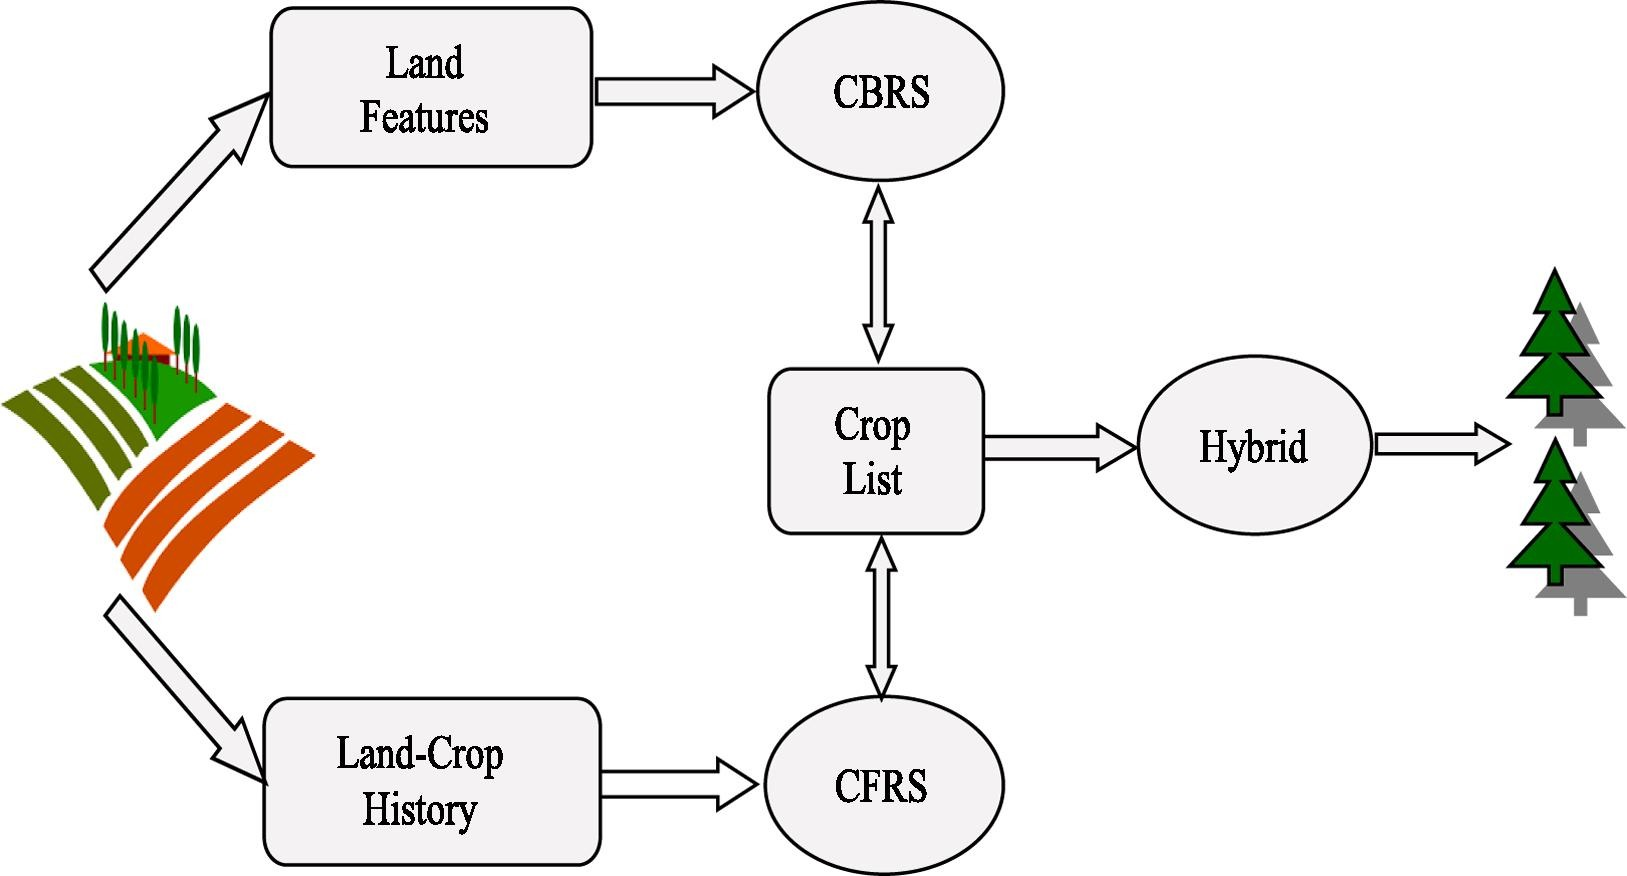
\includegraphics[width=\linewidth]{../graphics/Hybrid_RS_Land_Voorbeeld.jpg}
  \caption{Voorbeeld van hoe een hybride aanbevelingssysteem eruit kan zien \autocite{Patel2020}.} 
  \label{fig:hybrid_rs_land_voorbeeld}
\end{figure}

Het doel is een werkend proof-of-concept systeem te bouwen dat accurate en gepersonaliseerde aanbevelingen kan genereren, waarbij het vrijwel geen toegang heeft tot gevoelige gegevens van gebruikers. Door een combinatie van privacy behoudende technologieën, zoals FL en DP, vindt dit systeem een balans tussen bruikbaarheid en privacy. Als dit lukt, kan het een belangrijke stap zijn in de ontwikkeling van veilige en effectieve aanbevelingssystemen die vertrouwen winnen bij de gebruiker.

%---------- Stand van zaken ---------------------------------------------------
\section{Literatuurstudie}
\label{sec:literatuurstudie}

Aanbevelingssystemen zijn de laatste jaren enorm in opkomst en worden toegepast in verschillende sectoren. Ze zijn essentieel voor het bieden van gepersonaliseerde diensten aan gebruikers. Daarnaast vormen zulke diensten een effectieve inkomstenbron voor online bedrijven \autocite{Mazeh2020, Wang2018}. Echter, het gebruik van aanbevelingsdiensten vergt verzamelen van persoonlijke gegevens van gebruikers voor verwerking en analyse, wat gebruikers ongewenst vatbaar maakt voor privacyrisico's. Verder heeft elke serviceprovider een database met informatie over al zijn gebruikers \autocite{Wang2018, Lex2023, Yang2020, Friedman2015}.

Er zijn verschillende oplossingen uitgevonden om de privacy van gebruikers te beschermen. Eerste is Collaborative Filtering (CF), dit is een techniek die wordt gebruikt in aanbevelingssystemen om gebruikers te groeperen op basis van hun voorkeuren en interesses ten overzichte van andere gebruikers. Maar CF vereist een centrale server die de gegevens opslaat \autocite{Li2017,Wang2018}. Dit zorgt voor dat deze gebruikersgegevens kunnen worden misbruikt om privé informatie bekend te maken aan niet-vertrouwde partijen en om gebruikerskenmerken zoals geslacht of leeftijd af te leiden \autocite{Lex2023}. 
Differentional Privacy (DP) kan hierbij een oplossing bieden, uit \textcite{Friedman2015,Lex2023} volgt dat DP "is een rigoureus privacymodel dat ervoor zorgt dat de uitvoer van een berekening niet onthult of de gegevens van een specifieke persoon in de dataset zijn opgenomen". Dit wordt bereikt door zorgvuldig gekalibreerde ruis toe te voegen om de invloed van een enkele datapunt te maskeren.

Tweede techniek is Content Based (CB), aanbvelingssysteemen gebaseerd op CB bevelen items aan gebruikers aan op basis van de overeenkomsten tussen de inhoud van die items en voorkeuren van de gebruiker \autocite{Lops2010,Pazzani2007}. Hierbij worden verschillende datapunten van items en gebruikersprofielen geanalyseerd om patronen en voorkeuren te ontdekken en te groeperen. Hierin ligt ook het verschil met CF, waarbij de focus ligt op de overeenkomsten tussen gebruikers onderling. Nadelen van CB houden in: overspecialisatie, aanbevelingen hebben smal bereik van gebruikersinteresses, wat de ontdekking van nieuwe en diverse inhoud kan belemmeren en gedetailleerde analyse van gegevens, wat complex en tijdrovend kan zijn afhankelijk van de aard van de gegevens \autocite{Patel2020,Lops2010}.
In combinatie met Federated Learning (FL) kan CB verebterd worden. In plaats van gebruikersinformatie naar een centrale server te sturen, worden modellen getraind op het apparaat van de gebruikers zelf. Zo blijven persoonlijke gegevens lokaal bij de gebruiker en worden nooit uitgestuurd. Alleen geanonimiseerde modelupdates worden gedeeld met een centrale server, waardoor het systeem leert van de verzamelde inzichten zonder individuele gegevens te verzamelen \autocite{Wang2018, Lops2010}.

% Voor literatuurverwijzingen zijn er twee belangrijke commando's:
% \autocite{KEY} => (Auteur, jaartal) Gebruik dit als de naam van de auteur
%   geen onderdeel is van de zin.
% \textcite{KEY} => Auteur (jaartal)  Gebruik dit als de auteursnaam wel een
%   functie heeft in de zin (bv. ``Uit onderzoek door Doll & Hill (1954) bleek
%   ...'')

%---------- Methodologie ------------------------------------------------------ 

\section{Methodologie}%
\label{sec:methodologie}

We passen het strtegie van verdeel en heers om dit probleem makkelijker op te lossen. Beschouw het hybride aanbevelingssysteem als een combinatie van twee subsystemen: een Content Based (CB) gebaseerde en Collaborative Filtering (CF) gebaseerde systeem. 

Ten eerste zal er een uitgebreide literatuurstudie plaatsvinden, waarbij de huidige implementaties van CB en CF systemen worden onderzocht. Daarna gaan we na of er combinaties van deze systemen bestaan met Federated Learning (FL) en Differential Privacy (DP) technieken.
Vervolgens moeten de datasets verworven worden die tijdens het trainen en evalueren van het systeem worden gebruikt. De MovieLens 10M is een dataset, die meer dan 10 miljoen beoordelingen van meer dan 10.000 films door meer dan 71.000 gebruikers bevat. Deze dataset biedt zowel gebruikersbeoordelingen als informatie over de films zelf \autocite{Mazeh2020}.

Hierna volgt het prototype opbouwen van zowel het CF systeem met Differential Privacy als het CB systeem met Federated Learning. Deze prototypes zullen afzonderlijk worden getest en geëvalueerd op hun prestaties en privacybescherming. Voor elk systeem wordt gezocht naar een configuratie die voldoet aan de respectievelijk deelprobleem. Dit omvat het verfijnen van parameters en algoritmes om een oplossing te vinden die een goede balans biedt tussen aanbevelingskwaliteit en privacybescherming. Een oplossing wordt als geschikt beschouwd wanneer de gegenereerde aanbevelingen nauw aansluiten bij de referentievoorbeelden in de dataset. Dit geeft aan dat het systeem zowel relevant als effectief is in zijn aanbevelingen. Ten slotte wordt de Weighted Hybrid methode gebruikt om de twee systemen te integreren. Hierbij worden de aanbevelingen van beide systemen gecombineerd door gewichten toe te kennen aan de relatieve invloed van elk systeem, om zo tot een uiteindelijke aanbevelingen te komen.

Tot slot wordt het gecombineerde resultaat geëvalueerd in termen van algemene prestaties en privacyimpact door het te testen op de datasets om de kwaliteit van de aanbevelingen en het niveau van privacybescherming te beoordelen. De resultaten van deze experimenten zullen worden geanalyseerd en vergeleken met bestaande methoden om de voordelen en mogelijke nadelen van het voorgestelde hybride systeem te identificeren. De bevindingen uit deze evaluaties zullen bijdragen aan de verdere optimalisatie en validatie van het proof-of-concept systeem.

%---------- Verwachte resultaten ----------------------------------------------
\section{Verwacht resultaat, conclusie}%
\label{sec:verwachte_resultaten}

Van het voorgestelde hybride aanbevelingssysteem wordt verwacht dat het nauwkeurige en gepersonaliseerde aanbevelingen kan genereren en tegelijkertijd de privacy van de gebruiker beschermt. Het gebruik van DP in het CF systeem zal naar verwachting een sterke bescherming bieden voor gebruikersgegevens. Tegelijkertijd maakt het gebruik van FL binnen het CB systeem dat modellen lokaal getraind kunnen worden, waardoor de privacy nog beter beschermd wordt.

Verder wordt verwacht dat het hybride systeem een balans vindt tussen de nauwkeurigheid van aanbevelingen en het mate van privacy bescherming. Dit zal worden geëvalueerd aan de hand van metrieken zoals relevantie en de invloed van privacymaatregelen op de kwaliteit van aanbevelingen.

De resultaten van dit onderzoek kunnen bijdragen aan de ontwikkeling van veilige en betrouwbare aanbevelingssystemen die het vertrouwen van de gebruiker vergroten en tegelijkertijd voldoen aan strengere privacy-eisen. Dit proof-of-concept kan een basis vormen voor verdere innovatie in privacybewuste aanbevelingstechnologieën binnen de entertainmentindustrie en daarbuiten.
